\documentclass{beamer}

\usepackage{epsfig}
\usepackage{kotex}
\usepackage{graphicx}
\usepackage{latexsym}
\usepackage{amssymb}
\usepackage{amsmath,amscd}
\usepackage{multirow} 
\usepackage{array}
\usepackage{caption}
\usepackage{rotating}
\usepackage{subfig}
\usepackage{color}
\usepackage{natbib}
\usepackage{rotating}
\usepackage{graphicx,lscape}
\usepackage{amsmath, amsthm, amssymb}
\usepackage{graphicx}
\usepackage{epsfig}
\usepackage{graphics,color, graphicx}
\usepackage{latexsym}
\usepackage{amssymb,amsmath,amscd}
\usepackage{fancyvrb,enumerate}
\usepackage{amsmath, amsthm, amssymb}
\usepackage{multirow}
\usepackage{mathtools}
\usepackage{verbatim} 
\usepackage{afterpage}
\usepackage[ruled,vlined]{algorithm2e}
\usepackage{hyperref}
\usepackage[flushleft]{threeparttable}

\DeclarePairedDelimiter\abs{\lvert}{\rvert}
\DeclarePairedDelimiter\norm{\lVert}{\rVert}
\long\def\comment#1{} 

%\newtheorem*{thm}{Theorem}
\newtheorem{thm}{Theorem}[section]
\newtheorem{cor}[thm]{Corollary}
\newtheorem{lem}[thm]{Lemma}
\newcommand{\rb}[1]{\raisebox{-.5em}[0pt]{#1}}
\renewcommand{\baselinestretch}{1.8}
\renewcommand{\mid}{\, | \ }
\newcommand{\eighth}{{\textstyle \frac{1}{8}}}

\def \bY { \mathbf{ Y } }
\def \bX { \mathbf{ X } }
\def \bU { \mathbf{ U } }
\def \bmu { \boldsymbol{ \mu } }
\def \bSigma { \boldsymbol{ \Sigma } } 
\def \bphi { \boldsymbol{ \phi } }
\def \bepsilon { \boldsymbol{ \epsilon } }
\def \bD { \boldsymbol{\mathcal{D}} }


\newcommand{\eqdis}{\overset{\mathrm{d}}{=\joinrel=}}
\newcommand{\ba}{\mbox{\boldmath $a$}}
\newcommand{\bg}{\mbox{\boldmath $g$}}
\newcommand{\bx}{\mbox{\boldmath $x$}}
\newcommand{\by}{\mbox{\boldmath $y$}}
\newcommand{\bd}{\mbox{\boldmath $d$}}
\newcommand{\bff}{\mbox{\boldmath $f$}}
\newcommand{\bz}{\mbox{\boldmath $z$}}
\newcommand{\bu}{\mbox{\boldmath $u$}}
\newcommand{\bv}{\mbox{\boldmath $v$}}
\newcommand{\bW}{\mbox{\boldmath $W$}}
\newcommand{\bI}{\mbox{\boldmath $I$}}
\newcommand{\bJ}{\mbox{\boldmath $J$}}
\newcommand{\bL}{\mbox{\boldmath $L$}}
\newcommand{\bQ}{\mbox{\boldmath $Q$}}
\newcommand{\bZ}{\mbox{\boldmath $Z$}}
\newcommand{\bV}{\mbox{\boldmath $V$}}
\newcommand{\bG}{\mbox{\boldmath $G$}}
\newcommand{\bdm}{\begin{displaymath}}
\newcommand{\edm}{\end{displaymath}}
\newcommand{\bnu}{\mbox{\boldmath $\nu$}}
\newcommand{\btau}{\mbox{\boldmath $\tau$}}
\newcommand{\biota}{\mbox{\boldmath $\iota$}}
\newcommand{\bbeta}{\mbox{\boldmath $\beta$}}
\newcommand{\bomega}{\mbox{\boldmath $\omega$}}
\newcommand{\btheta}{\mbox{\boldmath $\theta$}}
\newcommand{\bep}{\mbox{\boldmath $\epsilon$}}
\newcommand{\bdelta}{\mbox{\boldmath $\delta$}}
\newcommand{\balpha}{\mbox{\boldmath $\alpha$}}
\newcommand{\bxi}{\mbox{\boldmath $\xi$}}
\newcommand{\bgamma}{\mbox{\boldmath $\gamma$}}
\newcommand{\bOmega}{\mbox{\boldmath $\Omega$}}
\newcommand{\bPi}{\mbox{\boldmath $\Pi$}}
\newcommand{\bzeta}{\mbox{\boldmath $\zeta$}}
\newcommand{\bpsi}{\mbox{\boldmath $\psi$}}
\newcommand{\bPsi}{\mbox{\boldmath $\Psi$}}
\newcommand{\bl}{\mbox{\boldmath $l$}}
\newcommand{\C}{{\rm Cov}}
\newcommand{\bH}{\bold H}
\newcommand{\blambda}{\mbox{\boldmath $\lambda$}}
\newcommand{\bbh}{\bld h}

\usetheme{metropolis}
%\usetheme{default}
%%\usecolortheme{lily}

\usefonttheme[onlymath]{serif}	% 수식 설정!!

\title{Bootstrap aggregated classification for sparse functional data}
%\date{\today}
\date[Short Occasion]{July 24, 2020}
\author{Hyunsung Kim}
\institute[Deptartment of Statistics]
	{Department of Statistics\\
 	 Chung-Ang University}

% A subtitle is optional and this may be deleted
%\subtitle{소제목}

%\author{F.~Author\inst{1} \and S.~Another\inst{2}}
% - Give the names in the same order as the appear in the paper.
% - Use the \inst{?} command only if the authors have different
%   affiliation.

%\institute[Universities of Somewhere and Elsewhere] % (optional, but mostly needed)
%{
%  \inst{1}%
%  Department of Computer Science\\
%  University of Somewhere
%  \and
%  \inst{2}%
%  Department of Theoretical Philosophy\\
%  University of Elsewhere}
% - Use the \inst command only if there are several affiliations.
% - Keep it simple, no one is interested in your street address.

%\date{Conference Name, 2013}
% - Either use conference name or its abbreviation.
% - Not really informative to the audience, more for people (including
%   yourself) who are reading the slides online

\subject{Bootstrap aggregated classification for sparse functional data}
% This is only inserted into the PDF information catalog. Can be left
% out. 

% If you have a file called "university-logo-filename.xxx", where xxx
% is a graphic format that can be processed by latex or pdflatex,
% resp., then you can add a logo as follows:

% \pgfdeclareimage[height=0.5cm]{university-logo}{university-logo-filename}
% \logo{\pgfuseimage{university-logo}}

% Delete this, if you do not want the table of contents to pop up at
% the beginning of each subsection:
%\AtBeginSubsection[]
%{
%  \begin{frame}<beamer>{Outline}
%    \tableofcontents[currentsection,currentsubsection]
%  \end{frame}
%}

% Let's get started
\begin{document}

\begin{frame}
  \titlepage
\end{frame}

\begin{frame}{Outline}
	\setbeamertemplate{section in toc}[circle]
%	\setbeamertemplate{subsection in toc}[ball unnumbered]
	\tableofcontents
	% You might wish to add the option [pausesections]
\end{frame}


\section{Introduction}

\begin{frame}{Introduction}
	\begin{itemize}
		\item{
			Functional data is collected in the form of curves or functions in various fields such as meteorology and health science, among others and analyzing this is called functional data analysis (FDA).
		}
		\item{
			Since functional data are defined on infinite dimensions, dimensionality reduction becomes a key issue and one of the powerful method is functional principal component analysis (FPCA) \citep{Silverman1996}.
		}
		\item{
			In real-data analysis, functional data are commonly observed at sparse or irregular time points, therefore \cite{James2000} and \cite{Yao2005} proposed the FPCA method for sparse functional data with different ideas.
		}
	\end{itemize}
\end{frame}

\begin{frame}{Introduction}
	\begin{itemize}
		\item{
			Similar to conventional multivariate data analysis, classifying into several groups is also important problem in FDA and there are some related works.
		}
		\item{
			\cite{Lee2004} presented a support vector machine (SVM) based on FPC scores, and \cite{Rossi2006} proposed a functional SVM (FSVM), extending the SVM for functional data.
		}
		\item{
			\cite{Song2008} compared classifiers based on FPC scores using linear discriminant analysis (LDA), quadratic discriminant analysis (QDA), a $k$-nearest neighbor (KNN) classifier, and SVM.
		}
		\item{
			\cite{Gama2004} proposed a functional tree model and bootstrap aggregating (bagging) functional trees.
		}
%		\item{
%			\cite{James2001} proposed a functional linear discriminant analysis (FLDA) for sparse functional data, implemented using an expectation-maximization (EM) algorithm.
%		}
%		\item{
%			\cite{James2002} and \cite{Muller2005} extended a generalized linear model to a functional analogue.
%		}
%		\item{
%			\cite{Leng2006} applied a functional logistic regression based on FPC scores to temporal gene expression data and compared the results with those of the B-spline basis method.
%		}
	\end{itemize}
\end{frame}

\begin{frame}{Introduction}
	\begin{itemize}
		\item{
			In this study, we propose a new classification method for sparse functional data based on FPCA and bootstrap aggregating.
		}
		\item{
			Bagging is an ensemble method that enhances predictions by combining the classifiers from the bootstrap samples.
		}
		\item{
			By extending the bagging to functional data, we construct a bagged classification model, which combines classifiers based on the FPC scores from the bootstrap samples.
		}
	\end{itemize}
\end{frame}


\section{FPCA for sparse functional data}\label{ch2}

\begin{frame}{Functional principal component analysis}
	\begin{itemize}
		\item{
			$\left\{ X(t) : t \in \mathcal{T} \right\}$ : a square integrable random process in $L^2(\mathcal{T})$
			\begin{itemize}
				\item[$\triangleright$]{
					$\mu(t) = E\big[X(t)\big], ~~ t \in \mathcal{T}$
				}
				\item[$\triangleright$]{
					$G(s,t) = \text{cov}\big[X(s),X(t)\big], ~~ s, t \in \mathcal{T}$
				}
			\end{itemize}
		}
		\item{
			By Mercer's theorem, the covariance function can be represented as 
			$$G(s,t) = \sum_{k=1}^\infty \lambda_k \phi_k(s) \phi_k(t),$$ 
			where $\lambda_1 \ge \lambda_2 \ge \dots \ge 0 $ are nonnegative eigenvalues satisfying $\sum_{k=1}^\infty \lambda_k < \infty$, and $\phi_k$ is the corresponding orthonormal eigenfunction.
		}
	\end{itemize}
\end{frame}

\begin{frame}{Functional principal component analysis}
	\begin{itemize}
		\item{
			Given $n$ random curves, $\bX = [ X_1(t) , \ldots, X_n(t) ]$, the Karhunen--Lo\`{e}ve expansion of $X_i(t)$ can be represented as
			\begin{equation*}
				X_i(t) = \mu(t) + \sum_{k=1}^\infty \xi_{ik} \phi_k(t), \hspace{0.5cm} t \in \mathcal{T},
			\end{equation*}
			where $\xi_{ik} =\mathlarger{  \int}_{\mathcal{T} }  \big( X_i(t) - \mu(t) \big)\phi_k(t) dt $ are uncorrelated variables with mean 0 and variance $\lambda_k$. 
		}
	\end{itemize}
\end{frame}

\begin{frame}{Functional principal component analysis}
	\begin{itemize}
		\item{
			The truncated approximation is written as
			\begin{equation*}
			X_i(t) \approx \mu(t) + \sum_{k=1}^K \xi_{ik} \phi_k(t), \hspace{0.5cm} t \in \mathcal{T},
			\end{equation*}
			where $K$ is the number of basis functions.
		}
		\item{
			$K$ is often selected using the proportion of variance explained (PVE), but the Akaike information criterion (AIC) or Bayesian information criterion (BIC) can also be used for consistency \citep{Yao2005,Li2013}.
		}
	\end{itemize}
\end{frame}

\begin{frame}{FPCA for sparse functional data}
	\begin{itemize}
		\item{
			When each curve is observed at sparse or irregular time points, we cannot apply a conventional FPCA directly to the data.
		}
		\item{
			Especially, the covariance function cannot be computed easily and the estimated FPC scores are biased.
		}
		\item{
			\cite{James2000} proposed a reduced-rank model based on the mixed-effects model and estimated the FPC function and scores using an EM algorithm.
		}
		\item{
			\cite{Yao2005} proposed the principal component analysis through the conditional expectation (PACE) method to obtain unbiased FPC scores.
		}
		\item{
			Here, we consider PACE method.
		}
	\end{itemize}
\end{frame}

\begin{frame}{FPCA for sparse functional data by PACE}
	\begin{itemize}
		\item{
			 Consider an $i$th curve $\bX_i = \big( X_i(t_{i1}), \dots, X_i(t_{in_i}) \big)^T$ with the mean function $\bmu_i = \big( \mu(t_{i1}), \dots, \mu(t_{in_i}) \big)^T$.
		}
		\item{
			Here, $t_{ij} \in \mathcal{T}$ is the $j$th time point observed in the $i$th curve $X_i$, for $i = 1, 2, \dots, n$, $j = 1, 2, \dots, n_i$.
		}
		\item{
			Let $\bU_i = \big( U_i(t_{i1}), \dots, U_i(t_{in_i}) \big)^T$ be an observed $i$th curve with additional measurement errors, $\bepsilon_i = \big( \epsilon_i(t_{i1}), \dots, \epsilon_i(t_{in_i}) \big)^T$.
		}
	\end{itemize}
\end{frame}

\begin{frame}{FPCA for sparse functional data by PACE}
	\begin{itemize}
		\item{
			Then, we have
			\begin{eqnarray*}
				%\bY_i = \bmu_i + \sum_{k=1}^\infty \xi_{ik} \bphi_{ik} + \bepsilon_i.
				U_i(t_{ij})& =&X_i(t_{ij}) + \epsilon_i(t_{ij})\\
				& =&  \mu(t_{ij}) + \sum_{k=1}^\infty \xi_{ik} \phi_k(t_{ij}) + \epsilon_i(t_{ij}), \hspace{0.5cm} t_{ij} \in \mathcal{T},
			\end{eqnarray*}
			where $\epsilon_i(t_{ij})$ is an $i.i.d.$ error with mean zero and variance $\sigma^2$ and is assumed to be independent of $\xi_{ik}$, for $i = 1, 2, \dots, n$, $j = 1, 2, \dots, n_i$, $k=1, 2, \ldots $.
		}
	\end{itemize}
\end{frame}

\begin{frame}{FPCA for sparse functional data by PACE}
	\begin{itemize}
		\item{
			Under the assumption that $\xi_{ik}$ and $\epsilon_i$ are jointly Gaussian, the best linear unbiased prediction (BLUP) of $\xi_{ik}$ is computed as
			\begin{equation*}
			\tilde \xi_{ik} = E[\xi_{ik} \vert \bU_i] = \lambda_k \bphi_{ik}^T\bSigma_{\bU_i}^{-1}(\bU_i - \bmu_i), 
			\end{equation*}
			where $\bphi_{ik} = \big( \phi_k(t_{i1}), \dots, \phi_k(t_{in_i}) \big)^T$ is the $i$th FPC function, and $\bSigma_{\bU_i} = \text{cov}(\bU_i, \bU_i) = \text{cov}(\bX_i, \bX_i) + \sigma^2\mathbf{I}_{n_i}$.
		}
	\end{itemize}
\end{frame}

\begin{frame}{FPCA for sparse functional data by PACE}
	\begin{itemize}
		\item{
			\cite{Yao2005} considered the following prediction for the trajectory $X_i(t)$ using the first $K$ eigenfunctions:
			\begin{eqnarray*}
				\hat X_i(t) =\hat  \mu(t) + \sum_{k=1}^K \hat\xi_{ik} \hat \phi_k(t) ,
			\end{eqnarray*}
			where $\hat  \mu(t)$,  $\hat\xi_{ik}$, and  $\hat \phi_k(t) $ are estimations obtained from the entire data sample.
		}
	\end{itemize}
\end{frame}



\section{Ensemble classification via FPCA}

\begin{frame}{Classification with functional predictors}
	\begin{itemize}
		\item{
			To perform the classification for functional data, we consider the functional generalized linear model (FGLM) \citep{James2002, Muller2005}.
		}
		\item{
			Given the $i$th functional curve $X_i(t)$ and the corresponding response $y_i$, the FGLM can be represented as
			\begin{eqnarray}
			g(\mu) &= \alpha + \mathlarger{\int}_{\mathcal{T}} \beta(t) X_i(t) dt ,
			\label{fglm}
			\end{eqnarray}
			where $\mu = E(y_i | X_i)$, and $g(\cdot)$ is a link function. 
		}
		\item{
			Because we can only observe $X_i(t)$ at a finite time points $n_i$, the integral can be substituted by a summation. 
		}
	\end{itemize}
\end{frame}

\begin{frame}{Classification with functional predictors}
	\begin{itemize}
		\item{
			The estimate of the coefficient $\beta(\cdot)$ may be unstable because it is an extremely high-dimensional vector.
		}
		\item{
			We can solve this problem by expanding $\beta(\cdot)$ using a set of basis functions. 
		}
		\item{
			By employing an FPCA, we can use data-driven orthonormal basis functions to represent $\beta(\cdot)$.
		}
	\end{itemize}
\end{frame}

\begin{frame}{Classification based on FPC scores}
	\begin{itemize}
		\item{
			Let $\phi_k(t)$, for $k=1, 2, \ldots$, be an orthonormal basis function, and expand $X_i(t)$ and $\beta(t)$ as
			$$X_i(t) = \sum_{k=1}^K \xi_{ik} \phi_k(t), ~~~  \beta(t) = \sum_{k=1}^K \beta_k \phi_k(t)$$
			using the $K$-truncated FPCA model described in Section \ref{ch2}.
		}
		\item{
			Then, the FGLM in \eqref{fglm}
			 is represented as
			\begin{equation*}
			g(\mu) = \alpha + \sum_{k=1}^K \beta_k \xi_{ik}.
			\end{equation*}
		}
		\item{
			The estimation is stable because most of the variation can be expressed using a small number, $K$.
		}
	\end{itemize}
\end{frame}


\begin{frame}{Bootstrap aggregated functional classifier via sparse FPCA}
	\begin{block}{Bagging}
		\begin{itemize}
			\item{
				Bootstrap aggregating (Bagging) is a popular ensemble method that uses the bootstrap idea proposed by \cite{Breiman1996}.
			}
			\item{
				It extracts several samples with replacement and obtains the prediction by aggregating models from each bootstrap sample.
			}
		\end{itemize}
	\end{block}
\end{frame}

\begin{frame}{Bootstrap aggregated functional classifier via sparse FPCA}
	\begin{block}{Notations}
		\begin{itemize}
			\item{
				$\bD = \left\{ \left( \bU_i, y_i \right) : i=1, \dots, n \right\}$ : the set of sparse $n$ curves with $\bU_i = \big( U_i(t_{i1}), \dots, U_i(t_{in_i}) \big)^T$.
			}
			\item{
				$y_i \in \{1, \ldots, g\}$ : the response class label. \\
				(Here, we assume $g=2$)
			}
			\item{
				$\bD^{(b)} = \left\{ \left( \bU^{(b)}_i, y^{(b)}_i \right) : i=1, \dots, n \right\}$, for $b=1,\dots,B$ : a bootstrap resample from $\bD$. 
			}
		\end{itemize}
	\end{block}
\end{frame}

\begin{frame}{Bootstrap aggregated functional classifier via sparse FPCA}
	\begin{block}{Algorithm}
		\begin{enumerate}
			\item For $b = 1, \dots, B$, repeat
			\begin{enumerate}[(a)]
				\item Generate a bootstrap resample $\bD^{(b)}$ from the data $\bD$.
				\item Perform FPCA for $\bD^{(b)}$.
				\item Estimate the FPC scores by PACE and chose $K$ FPCs.
				\item Construct a classifier using $K$ FPC scores.
			\end{enumerate}
			\item Given a new curve $\bU^*(t)$,
			\begin{enumerate}[(a)]
				\item Estimate the FPC scores by PACE from $\bD^{(b)}$, for $b = 1, \dots, B$.
				\item Obtain the prediction $\hat f^{(b)}$ from the $b$th classifier constructed in step 1-(d), for $b = 1, \dots, B$.
			\end{enumerate}
			
			\item Obtain the final prediction $\hat y_{bag}$ aggregated from $\hat f^{(1)}, \dots, \hat f^{(B)}$.
		\end{enumerate}
	\end{block}
\end{frame}

\begin{frame}{Aggregating methods}
	\begin{block}{Majority vote}
		\begin{itemize}
			\item{
				The majority vote simply chooses the class that receives the highest total vote from all classifiers.
			}
			\item{
				The bagged classifier by the majority vote is 
				\begin{equation*}
				\hat y_{\text{bag}} = \arg\max_{ j \in \{1,2\} }  \frac{ \sum_{b=1}^B \mathbf I \big\{ \hat f^{(b)}(x) = j  \big\} }{B}, 
				\end{equation*}
				where $\mathbf I$ is the indicator function. 
			}
		\end{itemize}
	\end{block}
\end{frame}

\begin{frame}{Aggregating methods}
	\begin{block}{Out-of-bag (OOB) error weighted vote \citep{Pham2018}}
		\begin{itemize}
			\item{
				Let $e_b$, for $b=1, \dots, B$, be the OOB errors from $B$ bootstrapped models.
			}
			\item{
				By defining the weight as $w_b = 1/e_b$, the models that exhibit good performance receive higher weights.
			}
			\item{
				If $e_b = 0$, which means there are no errors from the OOB samples, we set $e_b = \min \{ e_1, \dots, e_{b-1}, e_{b+1}, \dots, e_B \}$.
			}
			\item{
				The bagged classifier using the OOB error weighted vote is
				\begin{equation*}
				\hat y_{\text{bag}} = \frac{\sum_{b=1}^B w_b \hat f^{(b)}(x)}{\sum_{b=1}^B w_b}.
				\end{equation*}
			}
		\end{itemize}
	\end{block}
\end{frame}


\section{Simulation studies}

\begin{frame}{Simulation 1}
	\begin{itemize}
		\item{
			We generate $N=200$ curves with two classes as 
			$$U_{gi}(t_{ij} ) = \mu_g(t_{ij} ) + \sum_{k=1}^3 \xi_{gk} \phi_k(t_{ij} ) + \epsilon_i(t_{ij} ),~~i=1, \ldots , 100, ~j=1, \ldots, n_{ij},$$
			where $g \in \{ 0,  1\}$ indicates a group label.
		}
		\item{
			The FPC functions are defined as
			\begin{eqnarray}
			\phi_k(t)=  \begin{cases}
			\cos(\pi kt /5) / \sqrt{5},~~ ~ k ~~\text{is odds}\\
			\sin(\pi kt /5) / \sqrt{5},~~ ~ k ~~\text{is even,}
			\end{cases}\label{sim1}
			\end{eqnarray}
		}
		\item{
			The FPC scores $\xi_{gk}$ are sampled from $i.i.d. \ N(0, \lambda_{gk})$, for $k=1,2,3$.
		}
		\item{
			The measurement error $\epsilon_i(t)$ is sampled from $i.i.d. \ N(0, 0.5^2)$.
		}
	\end{itemize}
\end{frame}

\begin{frame}{Simulation 1}
	\begin{table}[h!]
		\footnotesize
		\centering
		\caption{[Simulation 1] The parameters for three models.}\label{t1}
		\tabcolsep=11.5pt
		\begin{tabular}{lccc}
			\hline 
			Model & $g$ & $\mu_g(t)$ & $ (\lambda_{g1} ,\lambda_{g2},\lambda_{g3}) $ \\ 
			\hline
			\multirow{2}{*}{(A) Different means and variances} & 0 & $t + \sin(t)$ & $(4, 2, 1)$ \\
			& 1 & $t + \cos(t)$ & $(16, 8, 4)$ \\
			\hline
			\multirow{2}{*}{(B) Different means } & 0 & $t + \sin(t)$ & $(4, 2, 1)$ \\
			& 1 & $t + \cos(t)$ & $(4, 2, 1)$ \\
			\hline
			\multirow{2}{*}{(C) Different variances} & 0 & $t + \sin(t)$ & $(4, 2, 1)$ \\
			& 1 & $t + \sin(t)$ & $(16, 8, 4)$ \\
			\hline 
		\end{tabular}
	\end{table}
\end{frame}

\begin{frame}{Simulation 1}
	\begin{itemize}
		\item{
			To make each curve sparse, the number of observations for the $i$th curve, $n_i$, is randomly selected from $\{5, 6, \ldots, 10\}$, and the corresponding time points $t_{ij}$, for $j=1, \dots, n_i$, are selected from $i.i.d. \ Uniform(0, 10)$.
		}
		\item{
			For validation, we randomly split the generated data into a training and a test set, with 100 elements in each.
		}
		\item{
			We compare the results of the proposed method with those of six single functional classification models: logistic regression, SVM with linear kernel, SVM with gaussian kernel, LDA, QDA, and naive Bayes.
		}
	\end{itemize}
\end{frame}

\begin{frame}{Simulation 1}
	\begin{table}[h!]
		\footnotesize
		\centering
		\caption{The average classification errors (\%) and standard errors (in parentheses) from 100 Monte Carlo repetitions for three designs of simulation 1.}\label{t2}
		\tabcolsep=5pt
		\tiny
		\begin{tabular}{cccccccc}
			\hline\hline
			&        & Logistic   & SVM      & SVM        &   \multirow{2}{*}{LDA}  &  \multirow{2}{*}{QDA}   & Naive \\
			Model & Method & Regression & (Linear) & (Gaussian) &  &  & Bayes \\ 
			\hline
			\multirow{3}{*}{(A)} & Single        & 17.13 (4.86) & 17.03 (5.22) & 14.86 (5.26) & 16.38 (4.93) & 14.94 (5.20) & 16.12 (4.64) \\ 
			& Majority vote & 14.98 (4.15) & 15.24 (4.29) & 12.81 (4.50) & 15.03 (4.11) & 13.55 (4.47) & 14.98 (4.21) \\ 
			& OOB weight    & 14.80 (3.95) & 14.83 (4.10) & \textbf{12.56 (4.33)} & 14.83 (4.00) & 13.02 (4.16) & 14.39 (4.02) \\ 
			\hline
			\multirow{3}{*}{(B)} & Single        & 11.42 (3.44) & 10.89 (3.47) & 11.60 (3.99) & 10.71 (3.48) & 12.19 (3.50) & 13.56 (4.23) \\ 
			& Majority vote & 10.24 (3.24) & 10.14 (3.21) & 10.68 (3.57) & 10.04 (3.12) & 11.16 (3.33) & 12.06 (3.35) \\ 
			& OOB weight    & 10.30 (3.23) & \textbf{9.97 (3.18)} & 10.52 (3.41) & 10.04 (3.10) & 11.03 (3.30) & 11.82 (3.31) \\ 
			\hline
			\multirow{3}{*}{(C)} & Single        & 50.43 (5.72) & 49.38 (5.60) & 32.48 (4.89) & 50.46 (5.73) & 30.90 (4.45) & 30.31 (4.51) \\ 
			& Majority vote & 49.62 (5.63) & 48.41 (6.16) & 31.11 (5.26) & 49.49 (5.70) & 30.70 (4.26) & 29.70 (4.42) \\ 
			& OOB weight    & 49.19 (5.78) & 48.20 (6.21) & 30.99 (5.32) & 49.01 (5.75) & 30.57 (4.18) & \textbf{29.59 (4.34)} \\ 
			\hline\hline
		\end{tabular}
		\begin{tablenotes}
			\item[1] * The minimum error rate is marked in bold.
		\end{tablenotes}
	\end{table}
\end{frame}

\begin{frame}{Simulation 2}
	\begin{itemize}
		\item{
			Simulation 2 is motivated by \cite{Yao2016}. 
		}
		\item{
			We generate $n=700$ curves as  
			$$U_{i}(t) = \sum_{k=1}^{50} \xi_{ik} \phi_k(t) + \epsilon_i(t),~~i=1, \ldots , n.$$
		}
		\item{
			The FPC functions are generated as in \eqref{sim1}, and the FPC scores, $\xi_{ik}$, are sampled from $i.i.d. \ N(0, k^{-3/2})$, for $k=1, \ldots, 50$.
		}
		\item{
			For the sparsity of the data, the number of observations for the $i$th curve, $n_i$, is randomly selected from $\{10, 11, \ldots, 20\}$, and the corresponding time points $t_{ij}$, for $j=1, \dots, n_i$, are selected from $i.i.d. \ Uniform(0, 10)$.
		}
		\item{
			The measurement error $\epsilon_i(t)$ is sampled from $i.i.d. \ N(0, 0.1)$.
		}
	\end{itemize}
\end{frame}

\begin{frame}{Simulation 2}
	\begin{itemize}
		\item{
			Now, we consider the following three models:
			\begin{align*}
			\text{(A)~~~} & f(U_i) = \exp(\langle \beta_1, U_i \rangle / 2) - 1, \\
			\text{(B)~~~} &f(U_i) = \arctan(\pi \langle \beta_1, U_i \rangle) + \exp(\langle \beta_2, U_i \rangle / 3) - 1, \\
			\text{(C)~~~} &f(U_i) = \arctan(\pi \langle \beta_1, U_i \rangle / 4),
			\end{align*}
			where $\langle f, g \rangle = \mathlarger{\int}_{\mathcal{T}}  f(t) g(t) dt $ for $f, g \in L^2(\mathcal{T})$.
		}
		\item{
			Here, $\beta_1(t) = \sum_{k=1}^{50} b_k \phi_k(t)$, where $b_k=1$ for $k=1,2$, $b_k=(k-2)^{-3}$ for $k=3, \ldots, 50$, and $\beta_2(t) = \sqrt{3/10}(t/5-1)$.
		}
	\end{itemize}
\end{frame}

\begin{frame}{Simulation 2}
	\begin{itemize}
		\item{
			The class label for each curve, $U_i$, is defined as  $y_i = \text{sign} \{ f(U_i) + \epsilon_i \}$, where $\epsilon_i \sim~i.i.d. \ N(0, 0.1).$
		}
		\item{
			We randomly split the generated data into 200 training curves and 500 test curves and compare the results of the proposed methods with those of the single classification models.
		}
	\end{itemize}
\end{frame}

\begin{frame}{Simulation 2}
	\begin{table}[ht]
		\footnotesize
		\centering
		\caption{The average classification errors (\%) and standard errors (in parentheses) from 100 Monte Carlo repetitions for three models in simulation 2.}\label{t3}
		\tabcolsep=5pt
		\tiny
		\begin{tabular}{cccccccc}
			\hline\hline
			&        & Logistic   & SVM      & SVM        &   \multirow{2}{*}{LDA}  &  \multirow{2}{*}{QDA}   & Naive \\
			Model & Method & Regression & (Linear) & (Gaussian) &  &  & Bayes \\ 
			\hline
			\multirow{3}{*}{A} & Single        & 16.71 (2.33) & 16.82 (2.20) & 17.50 (2.76) & 16.62 (2.30) & 17.77 (2.56) & 18.41 (2.66) \\ 
			& Majority vote & 15.62 (1.95) & 15.86 (1.87) & 16.19 (2.28) & 15.79 (1.96) & 16.51 (2.14) & 17.32 (2.42) \\ 
			& OOB weight    & \textbf{15.54 (1.93)} & 15.78 (1.83) & 16.17 (2.27) & 15.73 (1.89) & 16.43 (2.10) & 17.21 (2.40) \\ 
			\hline
			\multirow{3}{*}{B} & Single        & 12.85 (2.41) & 12.79 (2.40) & 13.27 (2.65) & 12.77 (2.40) & 13.83 (2.56) & 14.77 (2.74) \\ 
			& Majority vote & 11.20 (1.84) & 11.14 (1.89) & 11.54 (1.98) & 11.19 (1.85) & 11.93 (2.03) & 13.29 (2.36) \\  
			& OOB weight    & 11.11 (1.87) & \textbf{11.00 (1.81)} & 11.46 (1.94) & 11.11 (1.85) & 11.83 (2.00) & 13.08 (2.35) \\ 
			\hline
			\multirow{3}{*}{C} & Single        & 14.46 (2.17) & 14.34 (2.18) & 15.27 (2.69) & 14.29 (2.17) & 15.32 (2.36) & 16.05 (2.22) \\ 
			& Majority vote & 13.15 (1.73) & 13.14 (1.78) & 13.62 (2.08) & 13.14 (1.82) & 13.78 (1.90) & 14.88 (2.09) \\  
			& OOB weight    & 13.11 (1.77) & \textbf{13.06 (1.77)} & 13.54 (2.02) & 13.09 (1.80) & 13.74 (1.89) & 14.72 (2.08) \\  
			\hline\hline
		\end{tabular}
		\begin{tablenotes}
			\item[1] * The minimum error rate is marked in bold.
		\end{tablenotes}
	\end{table}
\end{frame}


\section{Real-data analysis}

\begin{frame}{Real-data analysis - Berkely growth data}
	\begin{itemize}
		\item{
			The Berkely growth data set \citep{Tuddenham1954} includes heights for 93 individuals (54 girls and 39 boys).
		}
		\item{
			There are 31 observations from ages 1 to 18 for each curve.
		}
	\end{itemize}
	\begin{figure}[h]
		\centering
		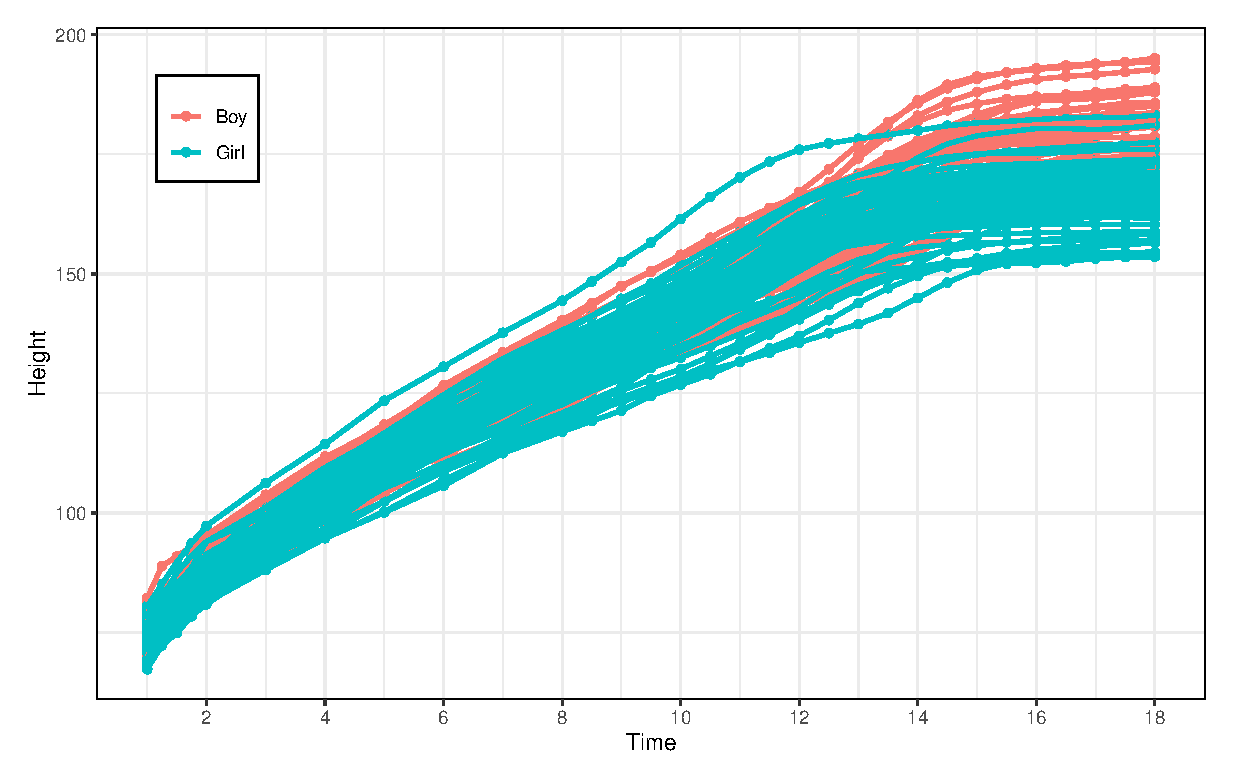
\includegraphics[height=4cm,keepaspectratio=true]{img/growth.eps}
		\caption{The Berkely growth data of 93 individuals.}	\label{fig1}
	\end{figure}
\end{frame}

\begin{frame}{Real-data analysis - Berkely growth data}
	\begin{itemize}
		\item{
			For sparseness, we artificially sparsify the data.
		}
		\item{
			The number of observations for each individual is randomly selected from $\{12,13, \ldots,  15\}$, and the corresponding time points are randomly selected from the original time points. 
		}
		\item{
			For validation, we randomly divide the 93 curves into 62 training and 31 test curves. 
		}
		\item{
			We repeat this process 100 times with different splits.
		}
	\end{itemize}
\end{frame}

\begin{frame}{Real-data analysis - Berkely growth data}
	\begin{table}[ht]
		\footnotesize
		\centering
		\caption{The average classification errors (\%) and standard errors (in parentheses) from 100 random splits of the Berkerly growth data.}\label{t4}
		\tabcolsep=6.5pt
		\tiny
		\begin{tabular}{ccccccc}
			\hline \hline
			& Logistic   & SVM      & SVM        &  \multirow{2}{*}{LDA}   &  \multirow{2}{*}{QDA}   & Naive \\
			Method & Regression & (Linear) & (Gaussian) &  &  & Bayes \\ 
			\hline
			Single        & 7.26 (4.80) & 5.26 (3.20) & 5.68 (4.03) & 5.81 (3.34) & 5.65 (3.35) & 5.65 (3.90) \\ 
			Majority vote & 5.94 (4.12) & 4.90 (3.19) & 5.26 (3.51) & 5.39 (3.24) & 4.87 (3.57) & 5.45 (3.96) \\ 
			OOB weight    & 6.06 (4.36) & 5.13 (3.11) & 5.32 (3.68) & 5.42 (3.24) & \textbf{4.87 (3.42)} & 5.39 (3.97) \\
			\hline \hline
		\end{tabular}
	\end{table}
\end{frame}

\begin{frame}{Real-data analysis - Spinal bone mineral density data}
	\begin{figure}[h]
		\centering
		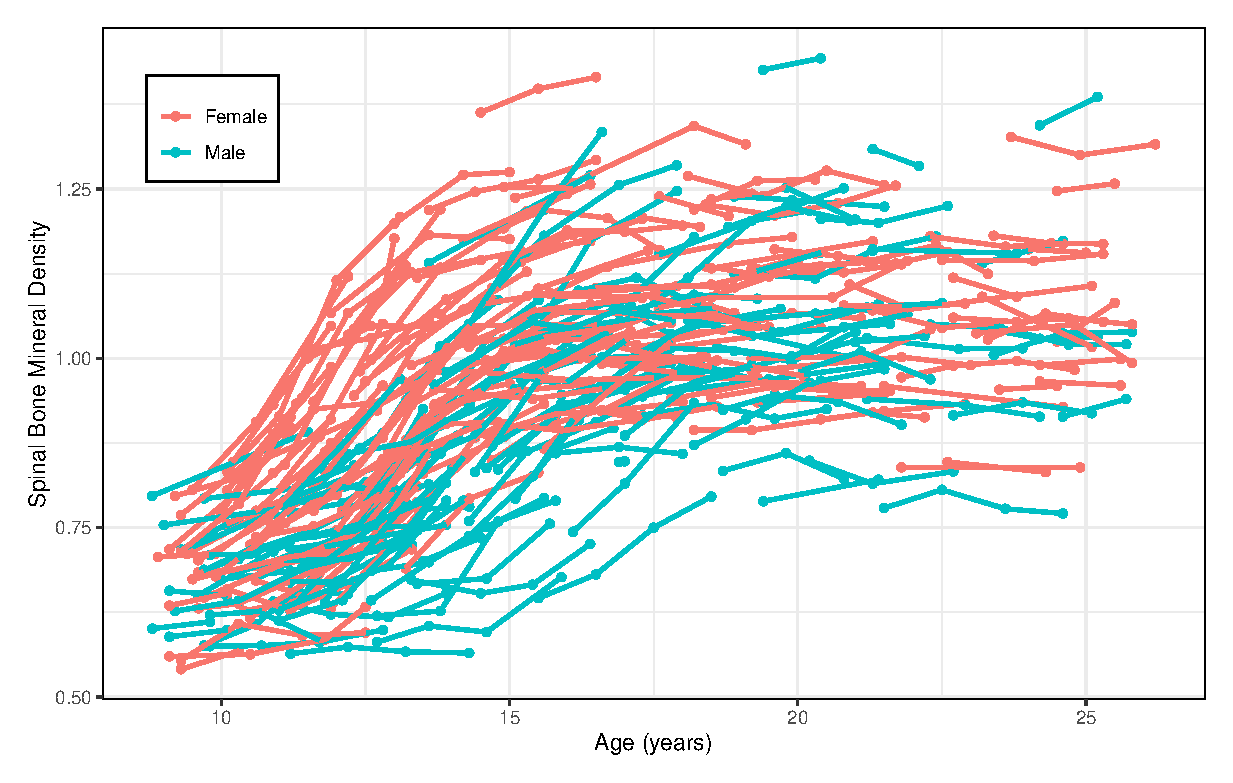
\includegraphics[height=4cm,keepaspectratio=true]{img/spnbmd.eps}
		\caption{The spinal bone mineral density of 280 individuals.}
		\label{fig2}
	\end{figure}
\end{frame}

\begin{frame}{Real-data analysis - Spinal bone mineral density data}
	\begin{itemize}
		\item{
			The spinal bone mineral density data \citep{Bachrach1999} contains spinal bone mineral densities for 280 individuals (153 females and 127 males).
		}
		\item{
			Each curve was measured at sparse and irregular time points with 2 to 4 observations.
		}
		\item{
			The data are randomly divided into 187 training and 93 test sets.
		}
		\item{
			we apply the methods to 100 different splits of the data.
		}
	\end{itemize}
\end{frame}

\begin{frame}{Real-data analysis - Spinal bone mineral density data}
	\begin{table}[ht]
		\footnotesize
		\centering
		\caption{The average classification errors (\%) and standard errors (in parentheses) from 100 random splits of the spinal bone mineral density data}\label{t5}
		\tabcolsep=5pt
		\tiny
		\begin{tabular}{ccccccc}
			\hline \hline
			& Logistic   & SVM      & SVM          &  \multirow{2}{*}{LDA}   &  \multirow{2}{*}{QDA}     & Naive \\
			Method & Regression & (Linear) & (Gaussian) &  &  & Bayes \\ 
			\hline
			Single        & 32.20 (4.15) & 32.22 (4.21) & 32.64 (4.05) & 31.90 (4.22) & 34.21 (4.25) & 32.58 (4.02) \\ 
			Majority vote & \textbf{31.12 (4.25)} & 31.39 (4.27) & 31.50 (4.56) & 31.16 (4.15) & 32.34 (3.90) & 31.29 (3.88) \\ 
			OOB weight    & 31.19 (4.15) & 31.45 (4.23) & 31.57 (4.44) & 31.28 (4.12) & 32.32 (3.95) & 31.27 (3.87) \\
			\hline \hline
		\end{tabular}
	\end{table}
\end{frame}


\section{Conclusion and discussion}

\begin{frame}{Conclusion and discussion}
	\begin{itemize}
		\item{
			In this study, we propose a new ensemble classification method for sparse functional data, which is a bagged model that combines classifiers based on FPC scores.
		}
		\item{
			To obtain FPC scores for sparse functinal data, we perform FPCA by PACE method.
%			Since observed curves are often sparse in real-data analyses, we use FPC scores estimated using the PACE method.
		}
		\item{
			We consider two aggregating methods, a majority vote and an OOB weighted vote, and find that both methods outperform the single classifiers.
		}
		\item{
			The results of several simulations confirm that the proposed classification model outperforms single classifiers in various situations.
		}
		\item{
			In two real-data analyses, the proposed model shows better performance than the single model.
%			Here, we also apply the proposed method to real data.
		}
	\end{itemize}
\end{frame}

\begin{frame}{Conclusion and discussion}
	\begin{itemize}
		\item{
			The proposed method can be easily extended to multi-class classification problems, in which we expect the aggregating method to outperform single classifiers. 
		}
		\item{
			In addition, other ensemble methods such as boosting and stacking can be used \citep{Opitz1999}.
		}
	\end{itemize}
\end{frame}



\section*{Reference}
\begin{frame}[allowframebreaks]
	\frametitle<presentation>{Reference}
	\renewcommand{\section}[2]{}   % delete "References" section title
	\begin{thebibliography}{9}
		\footnotesize
		
		\bibitem[{Bachrach et~al.(1999)}]{Bachrach1999}
		Bachrach, L. K., Hastie, T., Wang, M. C., Narasimhan, B., \& Marcus, R. (1999). Bone mineral acquisition in healthy Asian, Hispanic, black, and Caucasian youth: a longitudinal study. {\em The journal of clinical endocrinology \& metabolism}, {\bf 84}, 4702-4712.
		
		\bibitem[{Breiman(1996)}]{Breiman1996}
		Breiman, L. (1996). Bagging predictors. {\em Machine learning}, {\bf 24}, 123-140.
		
		\bibitem[{Breiman(1996)}]{Breiman1996b}
		Breiman, L. (1996). Out-of-bag estimation. Technical report, Statistics Dept., University of California at Berkeley, CA.
		
		\bibitem[{Ferraty and Vieu(2003)}]{Ferraty2003}
		Ferraty, F., \& Vieu, P. (2003). Curves discrimination: a nonparametric functional approach. {\em Computational Statistics \& Data Analysis}, {\bf 44}, 161-173.
		
		\bibitem[{Friedman et~al.(2001)}]{Friedman2001}
		Friedman, J., Hastie, T., \& Tibshirani, R. (2001). {\em The elements of statistical learning.}, Springer series in statistics, New York.
		
		\bibitem[{Gama(2004)}]{Gama2004}
		Gama, J. (2004). Functional trees. {\em Machine Learning}, {\bf 55}, 219-250.
		
		\bibitem[{Hall and Hosseini‐Nasab(2006)}]{Hall2006}
		Hall, P., \& Hosseini‐Nasab, M. (2006). On properties of functional principal components analysis. {\em Journal of the Royal Statistical Society: Series B (Statistical Methodology)}, {\bf 68}, 109-126.
		
		\bibitem[{James et~al.(2000)}]{James2000}
		James, G. M., Hastie, T. J., \& Sugar, C. A. (2000). Principal component models for sparse functional data. {\em Biometrika}, {\bf 87}, 587-602.
		
		\bibitem[{James and Hastie(2001)}]{James2001}
		James, G. M., \& Hastie, T. J. (2001). Functional linear discriminant analysis for irregularly sampled curves. {\em Journal of the Royal Statistical Society: Series B (Statistical Methodology)}, {\bf 63}, 533-550.
		
		\bibitem[{James(2002)}]{James2002}
		James, G. M. (2002). Generalized linear models with functional predictors. {\em Journal of the Royal Statistical Society: Series B (Statistical Methodology)}, {\bf 64}, 411-432.
		
		\bibitem[{Lee(2004)}]{Lee2004}
		Lee, H. J. (2004). Functional data analysis: classification and regression. Ph. D. Dissertation, Texas A\&M University.
		
		\bibitem[{Leng and Müller(2006)}]{Leng2006}
		Leng, X., \& Müller, H. G. (2006). Classification using functional data analysis for temporal gene expression data. {\em Bioinformatics}, {\bf 22}, 68-76.
		
		\bibitem[{Li et~al.(2013)}]{Li2013}
		Li, Y., Wang, N., \& Carroll, R. J. (2013). Selecting the number of principal components in functional data. {\em Journal of the American Statistical Association}, {\bf 108}, 1284-1294.
		
		\bibitem[{Müller(2005)}]{Muller2005a}
		Müller, H. G. (2005). Functional modelling and classification of longitudinal data. {\em Scandinavian Journal of Statistics}, {\bf 32}, 223-240.
		
		\bibitem[{Müller and Stadtmüller(2005)}]{Muller2005}
		Müller, H. G., \& Stadtmüller, U. (2005). Generalized functional linear models. {\em the Annals of Statistics}, {\bf 33}, 774-805.
		
		\bibitem[{Opitz and Maclin(1999)}]{Opitz1999}
		Opitz, D., \& Maclin, R. (1999). Popular ensemble methods: An empirical study. {\em Journal of artificial intelligence research}, {\bf 11}, 169-198.
		
		\bibitem[{Pham(2018)}]{Pham2018}
		Pham, H. T. (2018). Generalized weighting for bagged ensembles. Ph. D. Dissertation, Iowa State University.
		
		\bibitem[{Ramsay and Silverman(2005)}]{Ramsay2005}
		Ramsay, J. O., \& Silverman, B. W. (2005) {\em Functional Data Analysis}, 2nd ed., Springer Series in Statistics, New York.
		
		\bibitem[{Rossi and Villa(2006)}]{Rossi2006}
		Rossi, F., \& Villa, N. (2006). Support vector machine for functional data classification. {\em Neurocomputing}, {\bf 69}, 730-742.
		
		\bibitem[{Silverman(1996)}]{Silverman1996}
		Silverman, B. W. (1996). Smoothed functional principal components analysis by choice of norm. {\em The Annals of Statistics}, {\bf 24}, 1-24.
		
		\bibitem[{Song et~al.(2008)}]{Song2008}
		Song, J. J., Deng, W., Lee, H. J., \& Kwon, D. (2008). Optimal classification for time-course gene expression data using functional data analysis. {\em Computational biology and chemistry}, {\bf 32}, 426-432.
		
		\bibitem[{Tuddenham and Snyder(1954)}]{Tuddenham1954}
		Tuddenham, R. D., \& Snyder, M. M. (1954). Physical growth of California boys and girls from birth to eighteen years. {\em University of California publications in child development}, {\bf 1}, 183-364.
		
		\bibitem[{Yao et~al.(2005)}]{Yao2005}
		Yao, F., Müller, H. G., \& Wang, J. L. (2005). Functional data analysis for sparse longitudinal data. {\em Journal of the American Statistical Association}, {\bf 100}, 577-590.
		
		\bibitem[{Yao et~al.(2016)}]{Yao2016}
		Yao, F., Wu, Y., \& Zou, J. (2016). Probability-enhanced effective dimension reduction for classifying sparse functional data. {\em Test}, {\bf 25}, 1-22.
	\end{thebibliography}	
\end{frame}


\begin{frame}
	\begin{center}
		\huge
		\textbf{Thank You!}
	\end{center}
\end{frame}


\end{document}


